\documentclass[a4paper,10pt]{article}

\usepackage{ucs}
\usepackage[utf8]{inputenc}
\usepackage{amsmath}
\usepackage{babel}
\usepackage{fontenc}
\usepackage{graphicx}
\usepackage{textgreek}
\usepackage{subcaption}
\usepackage{amsthm}

\usepackage{hyperref}

\date{12/08/2019}

\begin{document}
 \subsection{Funzione d'attivazione sticastica}
 La funzione d'attivazione gioca un ruolo fondamentale nel training delle rete neurali in quanto introduce la non linearit\'a indispensabile per poter approssimare una qualsiasi funzione. Tra le diverse descritte in precedenza ci concentriamo sulla ReLU, in particolare la funzione d'attivazione che sar\'a descritta prende in considerazione il valore ottenuto con la precedente e ci applica un rumore stocastico. In questo modo si riesce a prevenire meglio l'overfitting senza dover intervenire su quanto gi\'a appreso dalla rete durante il training. 
 Inizialmente si utilizzavano come funzione d' attivazione la sigmoide o la tangente iperbolica, in quanto continue, monotone e con condominio limitato. Il problema principale \'e dato dal fatto che le derivate tendono velocemente a valori molto piccoli, rallentando il processo di apprendimento. Per questo motivo la funzione ReLU \'e diventata particolarmente popolare e per comodit\'a la riprendiamo di seguito:
 \begin{equation} 
  ReLU\left(x\right) = max\left(x\right). 
 \end{equation} 
 E la sua derivata  \'e data da:
 \begin{equation} 
  ReLU'\left(x\right) = \begin{cases} 
     1 & \mbox{se} \;\;\; x < 0 \\
     O & \mbox{altrimenti} 
 \end{cases} 
 \end{equation} 

 La ReLU risolve in parte il problema delle derivate, tuttavia si annulla per tutti i valori negativi producendo la "morte" del neurone. Per risolvere il problema sono state introdotte delle varianti della ReLU, come la Leaky ReLU [5], Parametric ReLU[6] e la Expoential Linear Unit [7]. 
 L'idea di utilizzare una funzione di attivazione stocastico viene dal comportamento degli impulsi nervosi, i cui picchi sono disturbati da effetti bio-meccanici [8]. La perturbazione indotta risulta essere particolarmente efficace nel prevenire l'overfitting durante il training. In particolare si introduce una nuova funzione d'attivazione il cui output produce una perturbazione stocastica; si propone poi un metodo per governare la perturbazione stocastica addestrando i parametri della distribuzione di probabilit\'a  attraverso la back-propagation e viene mostrato come questa funzione d'attivazione aumenti le performance della rete, in particolare nell'ambito di "Visual object classification". 
 In figura \ref{ProbActEffectpng} visualizziamo i principali effetti dovuti all'applicazione di questa nuova funzione d'attivazione. 
 \begin{figure}[h!]
  \centering
  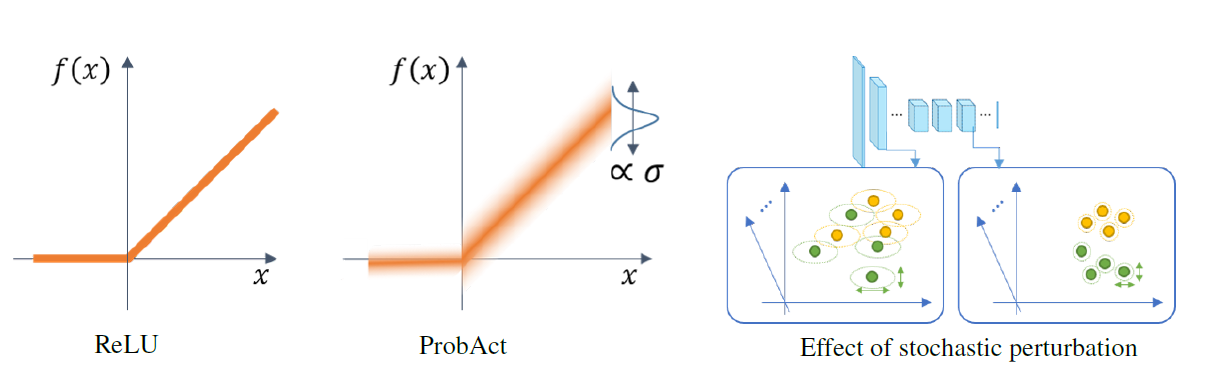
\includegraphics[width=\linewidth]{ProbActEffect.png} 
  \caption{da inserire}
  \label{ProbActEffectpng}
 \end{figure}

 In generale ogni layer di una rete neurale produce un output dato da:
 \begin{equation} 
  Y = f\left(w^{T} x\right), 
 \end{equation} 
 Dove $w^{T}$ indica il vettore dei pesi per quel layer, $x$ il vettore dell'input e $f$ la funzione d'attivazione, come pu\'o  essere la ReLU. Come mostrato in figura \ref{ProbActEffectpng} introduciamo una variabile randomica nella ReLU per creare una funzione d' attivazione stocastica. In particolare la si pu\'o definire come segue:
 \begin{equation} 
  f\left(x\right) = \mu \left(x\right) + z
 \end{equation} 
 Dove $\mu\left(x\right)$ \'e la ReLU e il tremine perturbativo $z$ pu\'o essere espresso come segue:
 \begin{equation} 
  z = \sigma  \epsilon. 
 \end{equation} 
 Il parametro perturbato $\sigma$ pu\' o essere fisso o addestrabile e definisce il renge della perturbazione stocastica ed $\epsilon$ \'e il valore ottenuto dalla distribuzione normale. Studiamo i casi in cui $\sigma$ sia fissa o addestrata. 
 Nel caso sia fissa, ci sono diversi modi per definirne il valore pi\'u adatto. Scegliendo ona $\sigma$ costante per tutti i valori \'e una opzione valida poich\'e $\epsilon$ \'e ottenuta randomicamente da una distribuzione normale e $\sigma$ funge da fattore di scala. La rete \'e ottimizzata usando l'apprendimento basato sul gradiente definito dal seguente teorema:
 \newtheorem{teorema}{Teorema}
 
 \begin{teorema} \label{GradienPropth}
  La propagazione del gradiente di una unit\'a stocastica h basata su una funzione deterministica g con input x (vettore contenente gli output dagli altri neuroni) e parametri interni $\phi$ (pesi e bias); se il rumore z \'e possibile e se g(x,$\phi$ ,z) ha gradiente non nullo allora\\
  
  \centering
  h = g(x, $\phi$ , z)
 \end{teorema}


 La natura di z \'e gaussiana, in quanto $z = \sigma \epsilon$ ed $\epsilon$ \'e effettivamente una variabile gaussiana. Ci\'o garantisce l'apprendimento attraverso il metodo basato sul gradiente. Il vantaggio principale di fissare $\sigma$ \'e quello di non aumentare il numero di parametri da dover addestrare nel training. 
 Si pu\'o comunque scegliere di lasciare $\sigma$ come parametro in pi\'u da addestrare durante il training tramite back-propagation, assieme agli altri parametri. Il calcolo del gradiente per $\sigma$ si ottiene attraverso la regola della catena. Data la funzione $F$, il gradiente di $F$ rispetto a $\sigma_{l, i}$ della $i$-esima unit\'a del $l$-esimo layer, \'e dato da:
 \begin{equation} 
  \frac{\partial F}{\partial\sigma_{l, i}} =  \frac{\partial F}{\partial y_{l, i}} \frac{\partial y_{l, i}}{\partial\sigma_{l, i}}
 \end{equation} 
 Con $y_{l, i}$ l'output dell'$i$-esima unit\'a del $l$-esimo layer. Il termine $\frac{\partial F}{\partial y_{l, i}}$ \'e il gradiente propagato dal layer pi\'u interno. Il gradiente dell' attivazione \'e dato da:
 \begin{equation} 
  \frac{\partial y_{l, i}}{\partial\sigma_{l, i}} = \epsilon
 \end{equation} 

 \begin{teorema} 
  Addestrare $\sigma$ senza porre dei limiti pu\'o provocare l'annullamento o la divergenza del parametro perturbativo con conseguente difficolt\'a nel training. Sfruttando le propriet\'a della funzione sigmoide possiamo definire $\sigma = \alpha sigmoid(\beta k)$ per avere $\sigma$ confinata tra $0$ e $\alpha$. Con $k$ il parametro da imparare e $\alpha$ e $\beta$ parametri che posso essere tenuti fissi. Negli esperimenti descritti di seguito avremo $\alpha = 2$ e $\beta = 5$ (valori scelti dopo un test apposito). S
 \end{teorema}

 Figura \ref{ProbActEffectpng} illustra gli effetti della perturbazione stocastica. Intuitivamente, la funzione d'attivazione stocastica aggiunge perturbazioni ad ogni passaggio tra un layer e quello successivo in modo indipendente, funzionando cos\'i anche come regolarizzatore della rete. Bisogna ricordare che il rumore viene poi propagato in tutti i layer successivi, quindi il rumore totale aggiunto ad un certo layer dipende dal rumore applicato in precedenza, ma anche dai pesi. Ad esempio, anche nel caso pi\'u semplice in cui la rete ha due layer con un ``neurone'' per ogni layer, la distribuzione dell'output $y_2$ del secondo layer differisce in base aai pesi del primo e secondo layer come segue:
 \begin{align}
  y_2 &= \mu \left[ w_2\mu\left(w_1 x\right) + w_2\sigma_1\epsilon\right] + \sigma_2\epsilon\\
  &= 
  \begin{cases}
   \mu\left[ w_2\mu\left(w_1 x\right)\right] + w_2\sigma_1\epsilon + \sigma_2\epsilon & \mbox{se} \;\; w_2\mu\left(w_1 x\right) + w_2\sigma_1\epsilon>0;\\
   \sigma_2\epsilon & \mbox{altrimenti}
  \end{cases} \\
  &\sim 
  \begin{cases}
   N\left(\mu\left[w_2\mu\left(w_1 x\right)\right],\left(w_2\sigma_1\right)^2 + \sigma_2^2\right)\\
   N\left(0,\sigma_2^2\right).
  \end{cases}
 \end{align}
 Come mostrato in figura \ref{ProbActEffectpng}, tender\'a ad essere appresa una piccola varianza del rumore nello strato finale, per fare in modo che l'output dela rete sia stabile. Utilizzando l'equazione del teorema \ref{GradienPropth} , consideriamo $g$ la funzione di introduzione del rumore nella rete, che dipende da $z$ e da alcune trasformazioni differenziabili $d$ sugli input $x$ e sui parametri interni del modello. Allora possiamo scrivere l'output $h$ come:
 \begin{equation}
  h = g(d,z) \label{outputh}
 \end{equation}
 Se utilizziamo l'equazione \ref{outputh} per altri metodi di aggiunta di rumore come il dropout [33] o per mascherare il rumore del denoising degli encoder automatici [34], si pu\'o dedurre $z$  come rumore moltiplicato subito dopo che la non linearit\'a \'e introdotta in un neurone. Nel caso dell'hash semantico [35], il rumore $z$ viene aggiunto poco prima della non linearit\'a. Nel caso descritto in questo documento, si campiona del rumore gaussiano e lo si aggiunge durante il calcolo di $h$. L'effetto della regolarizzazione \'e proporzionale alla varianza della distribuzione. Per evitare l'overfitting si pu\'o impostare un valore di varianza elevato.
 
 Valutiamo ora in alcuni esperimenti la funzione d'attivazione stocastica descritta in [aggiungere biblio], applicata alla classificazione di immagini. Mostriamo anche come tale funzione di attivazione lavori come regolarizzatore e come quindi pervenga l'overfitting. Descriviamo prima i dataset utilizzati e mostriamo di seguito i risultati:
 \begin{itemize}
  \item CIFAR-10 Dataset. 60000 immagini con 10 classi, 6000 immagini per classe e ogni immagine 32x32 pixel. 50000 immagini utilizzate per il training e 10000 per la convalida. 
  \item CIFAR-10 Dataset 100 classi e 600 immagini per classe. 500 immagini utilizzate per il training e le rimanenti per la convalida. La risoluzione anche per queste \'e di 32x32 pixel. 
  \item STL-10 Dataset. 500 immagini per ognuna delle 10 classi e 100 immagini tenute per il testing. Le immagini hanno una risoluzione di 96x96 pixel.
 \end{itemize}
 
 \begin{table}[h]\caption{da inserire}\label{ActFuncTestTab}
   \centering
   \begin{tabular}[h]{|l|c|c|c|c|c|}
    \hline
   Activation function & CIFAR-10 & CIFAR-100 & STL-10 & Train time & Test time \\ \hline
   ReLU & 86.67\% & 52.94\% & 60.80\% & \textbf{1.00 X ReLU} & \textbf{1.00 X ReLU} \\ 
   Leaky ReLU & 86.49\% & 49.44\% & 59.16\% & 1.04 X ReLU & 1.08 X ReLU \\
   PReLU & 86.35\% & 43.30\% & 60.01\% & 1.16 X ReLU & \textbf{1.00 X ReLU} \\
   Swish & 86.55\% & 54.01\% & 63.50\% & 1.20 X ReLU & 1.13 X ReLU \\
   \hline
   ProbAct & & & & & \\
   \quad Fixed ($\sigma$ = 0.5) & 88.50\% & 56.85\% & 62.30\% & 1.09 X ReLU & 1.25 X ReLU \\
   \quad Fixed ($\sigma$ = 1.0) & 88.87\% & \textbf{58.45}\% & 62.50\% & 1.10 X ReLU & 1.27 X ReLU \\
   \quad Single Trainable $\sigma$ & 87.40\% & 52.87\% & 63.07\% & 1.23 X ReLU & 1.30 X ReLU \\
   \quad Element-wise & 86.40\% & 53.10\% & 61.70\% & 1.25 X ReLU & 1.31 X ReLU \\
   \qquad Trainable $\sigma$ (unbound)  & & & & & \\
   \quad Element-wise & \textbf{88.92}\% & 55.83\% & \textbf{64.17}\% & 1.26 X ReLU & 1.33 X ReLU \\
   \qquad Trainable $\sigma$ (bound)  & & & & & \\
   \hline
   \end{tabular}
  \end{table}
  
  Per valutare le performance del metodo proposto si confronta la funzione d' attivazione $ProbAct$ con: ReLU, LeakyReLU, PReLU, e Swosh[9]. Si utilizza una rete a 16 layer Visual Geometry Group (VGG). Non vengono utilizzati metodi di regolarizzazione ulteriori o per-training o data augmentation. Gli input vengono normalizzati. Le immagini tratte da STL-10 sono state ridotte di soluzione per ottenere sempre immagini 32x32.
  I risultati mostrati in tabella \ref{ActFuncTestTab} sono ottenuti dalla media di 3 training differenti. Nel caso di $\sigma$ wide-trainable e bounded sono stati ottenuti risultati superiori del 2. 25\% su CIFAR-10, del 2. 89\% su CIFAR-10 e del 3. 37\% su STL-10, comparati con la ReLU. In aggiunta il metodo proposto risulta il migliore tra quelli confrontati.
  In figura \ref{SigmaTrainingpng} \'e mostrato l' andamento del training di $\sigma$. 
  \begin{figure}[h!]
   \centering
   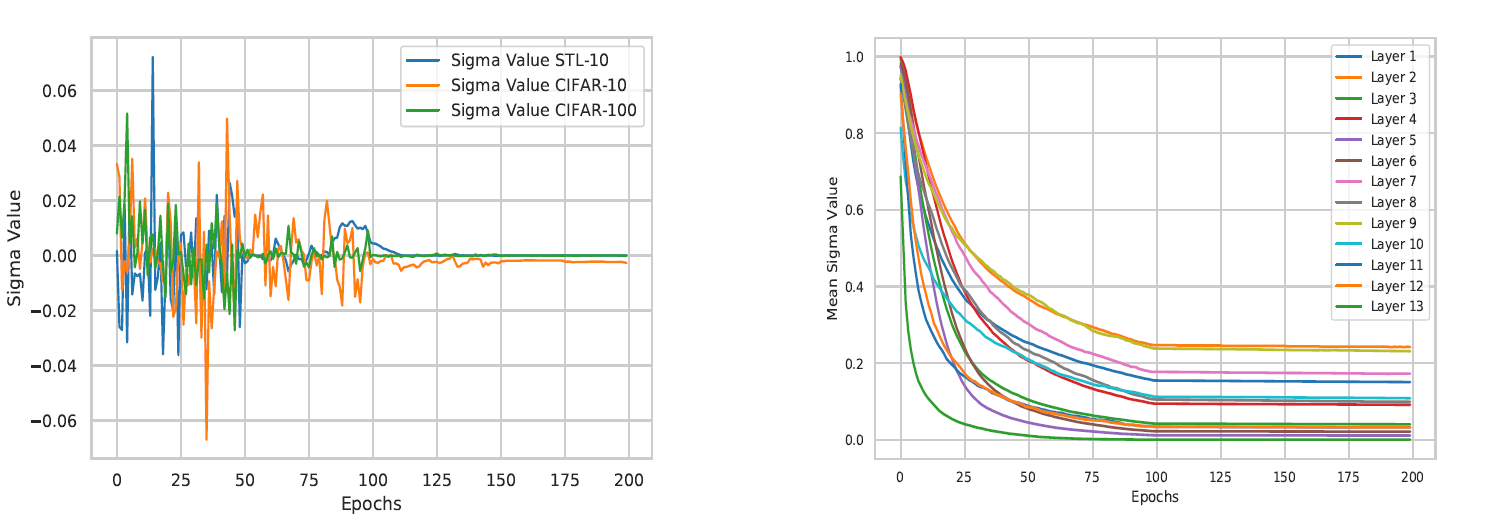
\includegraphics[width=\linewidth]{SigmaTraining.png} 
   \caption{da inserire}
  \label{SigmaTrainingpng}
  \end{figure}

  
  Il training \'e costituito da 400 epochs, ma non vengono mostrati i dati relativi alle epochs superiori a 200 in quanto non hanno contribuito significativamente al training. Infatti gi\'a dopo solo 100 epochs la $single$ $trainable$ $\sigma$ tende a 0. 
  Figura \ref{kFreqDistrpng} mostra la distribuzione in frequenza dell' elemento $k$ dopo 400 epochs. Osserviamo due picchi per ogni distribuzione attraverso i 3 dataset.  
  \begin{figure}[h!]
   \centering
   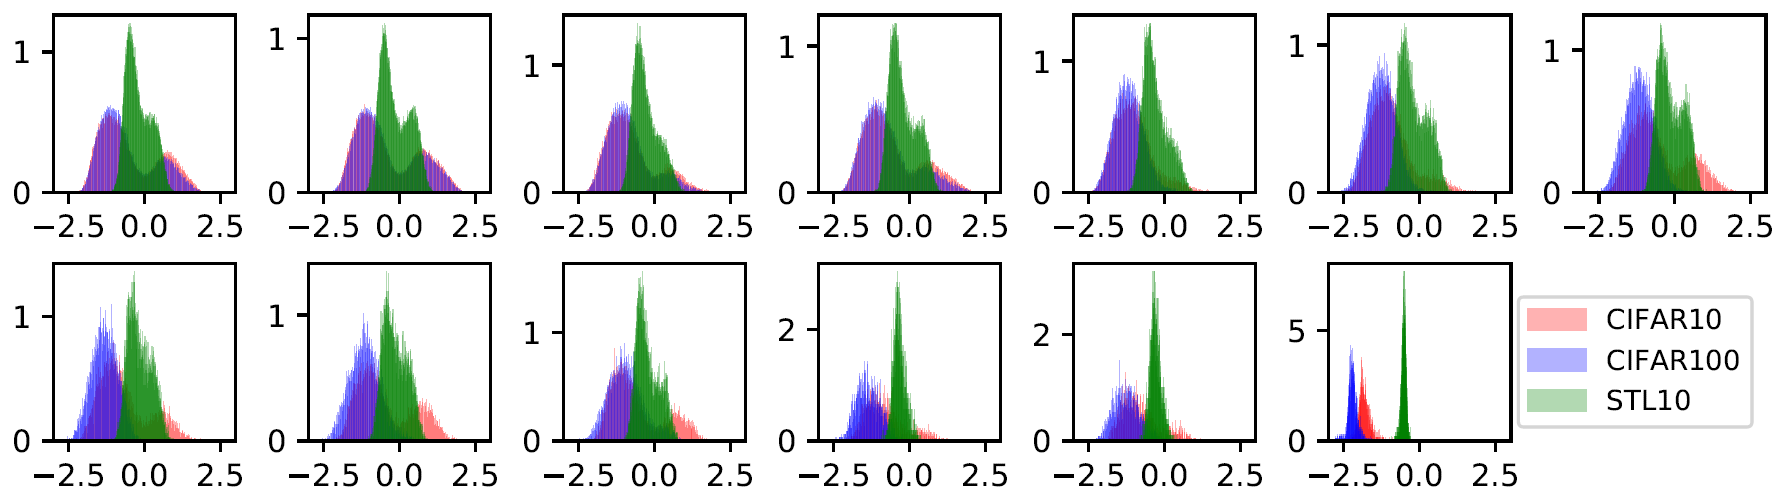
\includegraphics[width=\linewidth]{kFreqDistr.png} 
   \caption{da inserire}
  \label{kFreqDistrpng}
  \end{figure}
  
  Un elevato valore di $\sigma$ agisce come un regolarizzatore interno, migliorando la generalizzazione e prevenendo l'overfitting. Per definire il livello di overfitting di una rete utilizziamo un termine $\gamma$ che mostra la differenza di accuratezza tra training e test:
  \begin{equation}
   \gamma = TrainAccuracy(\%) - TestAccuracy(\%).
  \end{equation}
  
  Se $\gamma$ \'e piccolo, l'apprendimento in seguito al training si \'e generalizzato bene anche al set di test. Se invece \'e grande, la rete ha imparato molto bene a classificare gli esempi del training, ma non riesce a classificare casi diversi da quelli gi\'a visti. In figura \ref{WithWithoutDropoutpng} si confrontano le abilit\'a di generalizzazione con e senza l'utlizzo di dropout per il dataset CIFAR-100. 
  \begin{figure}[h!]
   \centering
   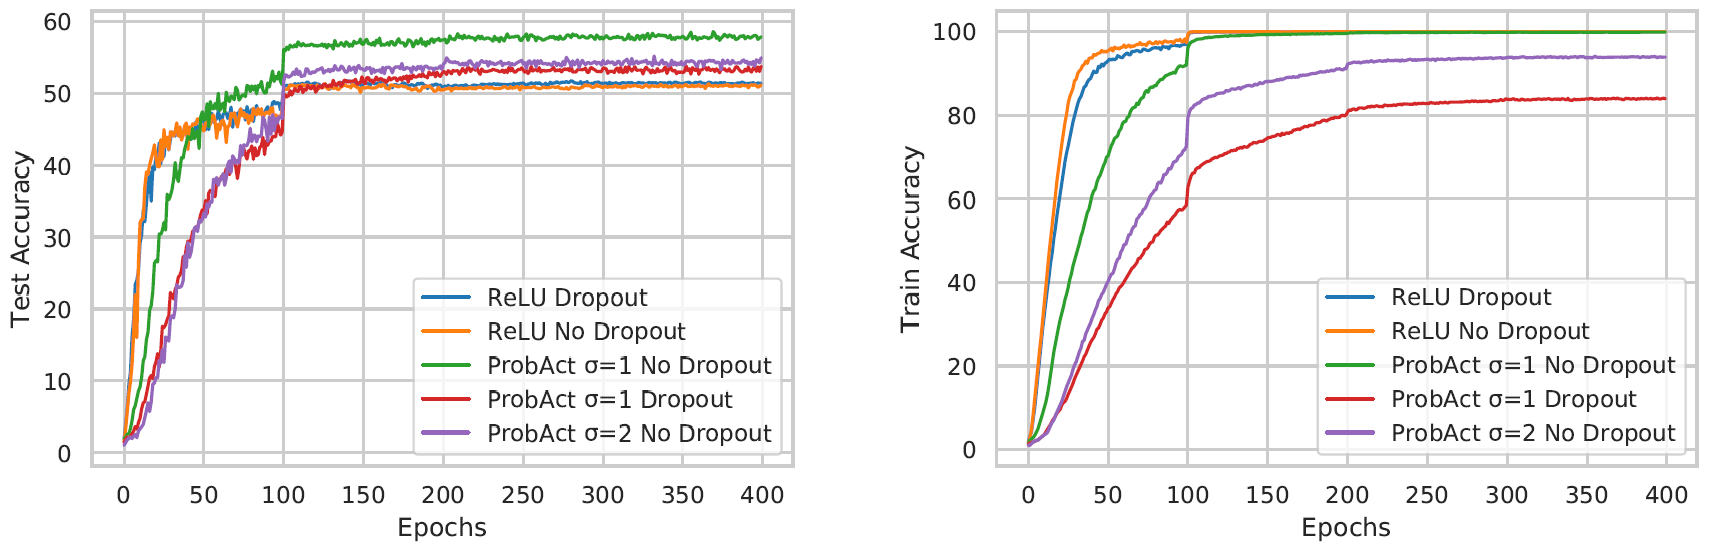
\includegraphics[width=\linewidth]{WithWithoutDropout.png} 
   \caption{da inserire}
  \label{WithWithoutDropoutpng}
  \end{figure} 
  
  
  Il dropout viene applicato con una probabilit\'a del 0.5\%. La rete senza dropout e con funzione d'attivazione ReLU ha circa $\gamma = 48\%$, valore che non viene modificato di molto se introdotto il dropout. D'altra parte, fissato $\sigma = 1$ si raggiunge $\gamma = 43\%$ e con $\sigma = 2$ si abbassa ulteriormente a $\gamma = 39\%$, sempre senza utilizzare il dropout. Introducendo anche il dropout si ottiene $\gamma = 30\%$ con $\sigma = 1$.
  Una funzione d'attivazione stocastica diventa particolarmente efficace nel caso in cui si abbia un dataset ridotto. Per confermare ci\'o sono stati confrontati i risultati di reti identiche, una con funzione d'attivazione ReLU e l'altra con funzione d'attivazione ProbAct, utilizzando solo una frazione dei dataset CIFAR-10 e CIFAR-100. I risultati ottenuti sono mostrati in tabella \ref{PartialDatasetTab}.
  \begin{table}[h]\caption{da inserire} \label{PartialDatasetTab}
   \centering
   \begin{tabular}[h]{|l|c|c|c|c|}
    \hline
    Activation function & CIFAR-10 (50\%) & CIFAR-100 (50\%) & CIFAR-10 (25\%) & CIFAR-100 (25\%) \\ \hline
    ReLU & 82.74\% & 42.36\% & 75.62\% & 30.42\% \\ 
    ProbAct & \textbf{84.73\%} & \textbf{46.11\%} & \textbf{79.02\%} & \textbf{31.67\%} \\ \hline
   \end{tabular}
  \end{table}
\end{document}
